\section{Auto Organização em RSSF}

 Auto organização é um processo pelo qual estrutura e funcionalidade (padrão) em nível global de um sistema emergem unicamente de numerosas interações entre componentes de baixo nível de um sistema sem qualquer controle externo ou centralizado. Os componentes do sistema interagem em um contexto local por meio de comunicação direta ou observações ambientais sem referência a um padrão global \cite{Dressler2008}.
 
 \subsection{Protocolos MAC auto organizáveis}
 
 A utilização de auto organização em redes de sensores sem fio possibilita ganhos em certos atributos dessas redes, como escalabilidade, consumo de energia, tolerância a falhas, etc. Em protocolos de acesso ao meio, auto organização é utilizada em mecanismos como: atribuição de recursos aos nós \cite{Dressler2008}, determinação de ciclos de sono%
 % FOOTNOTE begin 
 \footnote{Com o objetivo de aumentar o tempo de vida útil das RSSF são utilizados ciclos de sono (\textit{sleep-wakeup cycle} ou \textit{duty cycle}) onde cada nó é ligado apenas por um curto período de tempo (\textit{wakeup}) e então desligado novamente (\textit{sleep}). A utilização desses ciclos pode aumentar a vida útil das RSSF, devido à redução do consumo de energia durante o período de sono \textit{sleep}, de poucos dias para vários meses ou mesmo anos dependendo da razão entre o tempo em que o nó permanece ligado e o tempo em que permanece desligado.}
 % FOOTNOTE end
 \cite{Halkes:2005}, roteamento de pacotes, etc. Existem muitos exemplos de protocolos de controle de acesso ao meio que utilizam esse tipo de organização para diversos fins, abaixo estão apresentados alguns desses protocolos e o modo como a auto organização é empregada neles.
 
 \subsubsection{WiseMAC}
 
 WiseMAC é baseado em técnicas de amostragem de preâmbulo%
  % PREÂMBULO 
 \footnote{Preâmbulo é um fluxo de dados utilizado para comunicar a intenção de transmitir. Tem duração variável de acordo com o período de sono, pois é preciso garantir que o destinatário receba esse preâmbulo e identifique-se como receptor dos pacotes de dados que serão enviados em seguida.} 
 %
. Através da verificação periódica do meio em busca de atividades de comunicação \cite{El-Hoiydi2004}. Tal verificação consiste em uma varredura de curta duração do canal de rádio. Cada nó verifica o meio com um mesmo período constante \textit{Tw} (Figura ~\ref{fig:wisemac}). Se o meio está ocupado, o nó sensor continua a ouvi-lo até receber um quadro de dados ou até o meio ficar desocupado novamente. Antes de cada quadro de dados ser enviado, o ponto de acesso (\textit{access point}) envia um preâmbulo com a mesma duração do período de verificação para garantir que o receptor esteja acordado no momento em que o quadro de dados for enviado. 

\begin{figure}[!htb]
\centering
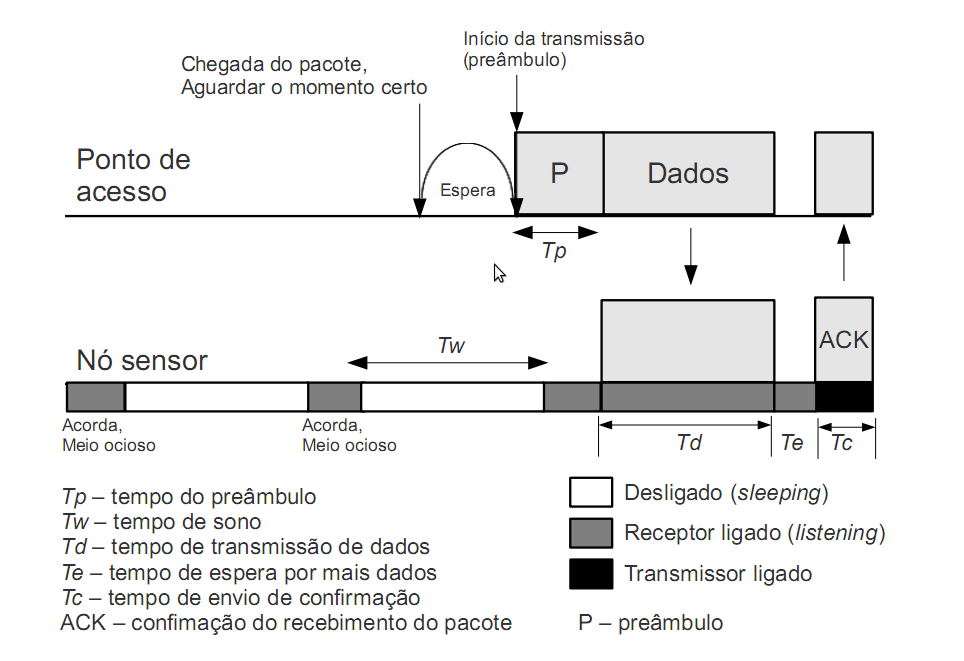
\includegraphics[width=340px,height=220px]{./Pictures/wisemac.png}
% SensorNodesScatteredInASensorField.png: 816x1056 pixel, 96dpi, 21.59x27.94 cm, bb=0 0 612 792
% pdfLaTeX aceita figuras no formato PNG, JPG ou PDF
% figuras vetoriais podem ser exportadas para eps e depois convertidas para pdf usando epstopdf
\caption{Funcionamento do WiseMAC \cite{El-Hoiydi2004}.} %legenda
\label{fig:wisemac} %rotulo para refencia
\end{figure}

Essa técnica promove um baixo consumo de energia quando o canal está desocupado, porém tem como desvantagem o fato de que os preâmbulos utilizados podem causar limitações à velocidade de transmissão entre pontos distantes e maior consumo de energia devido a sobrecarga nos receptores e ao fato de todos os nós permanecerem ouvindo essa transmissão (\textit{overhearing}). Um ganho considerável é conseguido ao fazer com que os pontos de acesso conheçam os ciclos de verificação dos outros nós pois ele poderá iniciar transmissões somente no momento em que os outros nós estarão ouvindo.

 \subsubsection{S-MAC}
 \label{sec:smac}
 
Sensor-MAC ou S-MAC foi desenvolvido para ter primordialmente baixo consumo de energia, além disso conseguiu-se também boa escalabilidade e baixo número de colisões \cite{ye04}. Para conseguir esse resultados foram tratados os seguintes problemas identificados pelo autor como responsáveis pelo consumo excessivo de energia na rede: colisões de pacotes, que causam a retransmissão desses pacotes e consequente consumo extra de energia além de aumentar a latência na rede; \textit{overhearing}, que acontece quando os nós recebem pacotes que não são destinados a eles; excesso (\textit{overhead}) de pacotes de controle; e \textit{idle listening}, quando um nó permanece em modo de recepção aguardando por pacotes que não são enviados.

Para alcançar esses resultados foi adotado um padrão de ciclos de sono com períodos longos de inatividade (período de sono) e períodos de atividade (\emph{duty cycle}) curtos. Auto organização está presente na sincronização dos períodos de atividade/sono dos nós em uma vizinhança, fazendo com que os nós adotem um mesmo cronograma de funcionamento. 

No momento em que cada nó é ligado, ele permanecerá ouvindo o meio com o objetivo de verificar a existências de nós vizinhos que já possuam agendas determinadas. Para que seja possível essa detecção, no início de seu \emph{duty cycle}, cada nó verifica o meio e, caso esteja desocupado, envia um pacote de sincronização (\emph{sync packet}) contendo informações da sua agenda. Os receptores desse pacote podem então adotar essa agenda e passam a possuir o mesmo \emph{duty cycle} do nó transmissor. 

Para evitar colisões no envio desses pacotes, antes de verificar a disponibilidade do meio para envio do \emph{sync packet} (Figura ~\ref{fig:SmacDutyCycle}), cada nó aguarda por um período de tempo aleatório. Esse período de espera é chamado período de contenção. 

\begin{figure}[!htb]
\centering
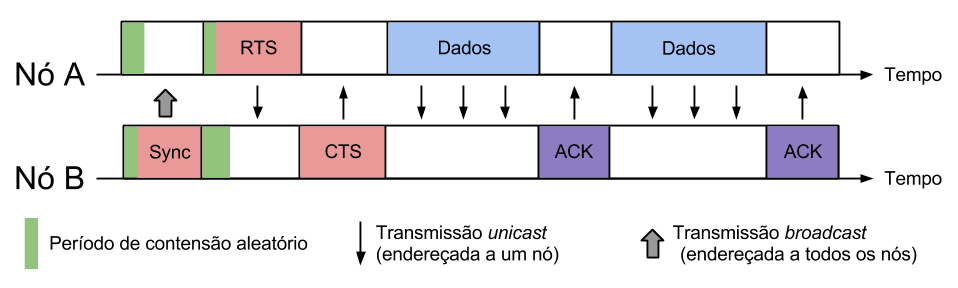
\includegraphics[width=360px,height=108px]{./Pictures/S-MACDutyCycle.png}
% SensorNodesScatteredInASensorField.png: 816x1056 pixel, 96dpi, 21.59x27.94 cm, bb=0 0 612 792
% pdfLaTeX aceita figuras no formato PNG, JPG ou PDF
% figuras vetoriais podem ser exportadas para eps e depois convertidas para pdf usando epstopdf
\caption{Funcionamento do \emph{duty cycle} no protocolo S-MAC.} %legenda
\label{fig:SmacDutyCycle} %rotulo para refencia
\end{figure}

A segunda parte do \emph{duty cycle} é reservada para transmissão e recepção de dois outros pacotes de controle que determinam se um nó pode enviar ou receber pacotes de dados. O primeiro desses pacotes é o RTS (\emph{Request To Send}). Um nó que deseja transmitir dados deve aguardar um novo período de contenção e então verificar novamente a disponibilidade do meio (Figura ~\ref{fig:SmacDutyCycle}). Caso o meio esteja disponível, ele enviará ao nó para o qual deseja transmitir um pacote RTS. Após receber um pacote RTS o nó receptor poderá enviar um pacote CTS (\emph{Clear To Send}) para notificar o transmissor que pode receber o pacote (Figura ~\ref{fig:SmacDutyCycle}). O nó não enviará o CTS nos casos onde já tenha ouvido um RTS ou CTS de um de seus vizinhos ou caso na sua vizinhança o meio esteja ocupado.

Após receber um CTS o nó transmissor aguarda o final do período de tempo reservado à transmissão dos pacotes de controle e então inicia a sua transmissão (Figura ~\ref{fig:SmacDutyCycle}). Ao final da transmissão, o no transmissões aguardará que seu receptor envie um pacote de confirmação de recebimento chamado ACK (\emph{Acknowledgement}). Após receber esse pacote, ele poderá continuar enviando pacotes de dados da mesma maneira. Caso o nó transmissor não receba um ACK, ele tentará reenviá-lo. Caso o nó não obtenha sucesso no envio de um pacote após algumas tentativas, o pacote poderá ser descartado.

Todo esse mecanismo possibilita que eles possam se comunicar com eficiência e se manterem sincronizados apesar do maior tempo de inatividade. Além disso, elimina a necessidade do uso de preâmbulos pois tem-se uma garantia de que os nós aos quais os dados se destinam estarão acordados no mesmo momento (ou em um momento muito próximo) em que aquele que deseja transmitir.

\begin{figure}[!htb]
\centering
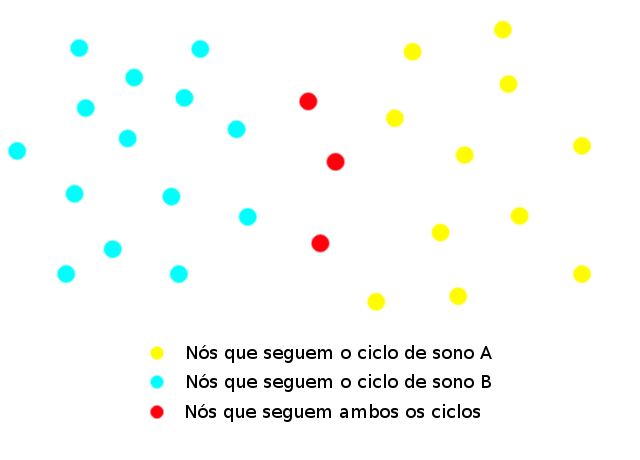
\includegraphics[width=290px,height=180px]{./Pictures/S-MACSynchronization.png}
% SensorNodesScatteredInASensorField.png: 816x1056 pixel, 96dpi, 21.59x27.94 cm, bb=0 0 612 792
% pdfLaTeX aceita figuras no formato PNG, JPG ou PDF
% figuras vetoriais podem ser exportadas para eps e depois convertidas para pdf usando epstopdf
\caption{Exemplo de sincronização de ciclos de atividades com protocolo S-MAC (\emph{clusters} A e B e nós de borda).} %legenda
\label{fig:SmacSynch} %rotulo para refencia
\end{figure}
 
Como desvantagem desse protocolo pode-se destacar que a sincronização dos ciclos de sono se dá entre um certo número de nós de uma região da rede e os nós que ficam no limiar entre duas regiões devem sincronizar-se com ambas as regiões (Figura ~\ref{fig:SmacSynch}). Isso faz com que o consumo de energia desses nós seja maior, reduzindo-se assim o seu tempo de vida útil.
 
 
\subsubsection{T-MAC} 

\citeauthoronline{vanDam:2003:AEM:958491.958512} (\citeyear{vanDam:2003:AEM:958491.958512}) apresentam o protocolo T-MAC. O T-MAC é um protocolo de controle de acesso ao meio baseado em contensão e, assim como o S-MAC, também utiliza \emph{duty cycles} e sincronização de nós. O que o diferencia do S-MAC é que o \emph{duty cycle} dos nós é adaptado de acordo com o tráfego da rede de sensores. O fim do período de atividades é determinado por um \emph{timeout}. Esse \emph{timeout} é configurado para que seja suficiente para a realização de um curto período de contenção e uma troca de pacotes RTS e CTS. 

Ao final desse período, caso o nó não tenha detectado nenhuma atividade no meio ele terminará seu \emph{duty cycle} e voltará a dormir. Caso o nó receba pacotes ou detecte o envio de pacotes entre seus vizinhos, ele irá iniciar um novo \emph{timeout} após o final desta comunicação (Figura ~\ref{fig:TmacDutyCycles}). 

Um problema encontrado nesse protocolo é que um nó que deseja transmitir um pacote, mas perde a contenção para um vizinho não comum, pemanecerá em espera até o final da transmissão desse vizinho. Ao final dessa transmissão, ele iniciará um novo \emph{timeout} e enviará um CTS, mas não receberá a resposta do nó destino, uma vez que ele não terá detectado a atividade do nó que venceu a contensão anterior.

\begin{figure}[!htb]
\centering
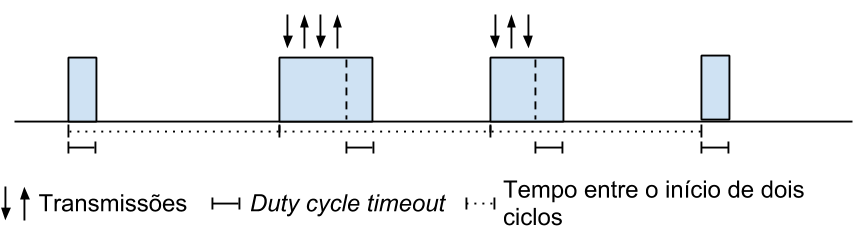
\includegraphics[width=290px,height=81px]{./Pictures/T-MACDutyCycles.png}
% SensorNodesScatteredInASensorField.png: 816x1056 pixel, 96dpi, 21.59x27.94 cm, bb=0 0 612 792
% pdfLaTeX aceita figuras no formato PNG, JPG ou PDF
% figuras vetoriais podem ser exportadas para eps e depois convertidas para pdf usando epstopdf
\caption{\emph{Duty cycle} adaptativo no protocolo T-MAC.} %legenda
\label{fig:TmacDutyCycles} %rotulo para refencia
\end{figure}

\subsubsection{D-MAC} 

O protocolo D-MAC, apresentado em \citeauthoronline{1303264} (\citeyear{1303264}), também utiliza \emph{duty cybcles} para reduzir o consumo de energia dos nós e aumentar o tempo de vida da rede. O que o diferencia dos outros protocolos apresentados é o modo como é feita a sincronização dos nós. 

Para o funcionamento desse protocolo é preciso que haja um nó concentrador (\emph{sync node}) conhecido. Assumindo-se que a maior parte da comunicação detro da rede será realizada em direção a esse nó concentrador, os nós são sincronizados a partir dele de forma que os nós que estejam a um número $n$ de saltos do nó concentrador iniciam seu \emph{duty cycle} um pouco depois dos nós que estão a uma distância em saltos igual a $n+1$ (Figura ~\ref{fig:DmacDutyCycles}).

Essa sincronização permite que transmissões de pacotes em direção ao nó concentrador partindo de qualquer ponto da rede tenham sua latência bastante reduzida. Cada pacote recebido por um nós do nível $n$ pode ser enviado para um nó do nível $n-1$ quase imediatamente.

O problema com esse protocolo é que ele só promove redução da latência de transmissão no sentido do gradiente em direção ao nó concentrador. Caso haja transmissões seguindo a direção contrária (como pacotes de requisição de dados), não haverá redução na latência dessas transmissões. 

\begin{figure}[!htb]
\centering
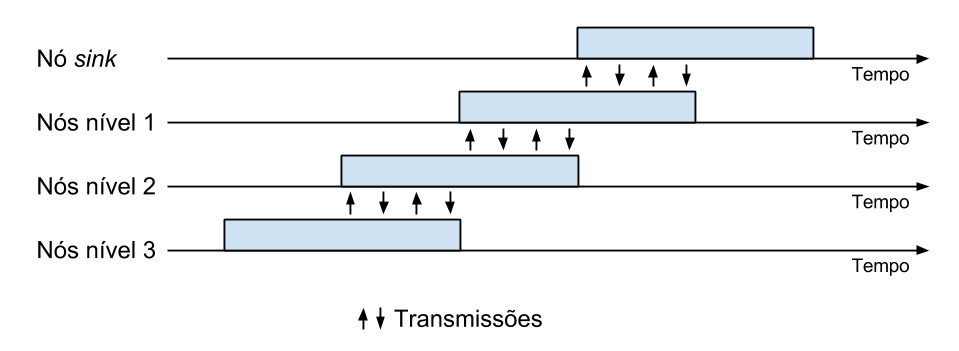
\includegraphics[width=290px,height=106px]{./Pictures/D-MACDutyCycles.png}
% SensorNodesScatteredInASensorField.png: 816x1056 pixel, 96dpi, 21.59x27.94 cm, bb=0 0 612 792
% pdfLaTeX aceita figuras no formato PNG, JPG ou PDF
% figuras vetoriais podem ser exportadas para eps e depois convertidas para pdf usando epstopdf
\caption{\emph{Duty cycle} sincronizado em níveis no protocolo D-MAC.} %legenda
\label{fig:DmacDutyCycles} %rotulo para refencia
\end{figure}